\documentclass[12pt,a4paper]{article}

% ---------------------------------------------------------------------------
% Kodiranje, jezik, fontovi
% ---------------------------------------------------------------------------
\usepackage[T1]{fontenc}
\usepackage[utf8]{inputenc}
\usepackage{lmodern}
% Napomena: babel sa srpskim (serbian.ldf) nije dostupan u svim TeX
% distribucijama, pa su nazivi (Slika, Tabela, Sadržaj...) postavljeni
% ručno radi prenosivosti. Na Overleaf-u se umesto ovoga može koristiti
% \usepackage[serbian]{babel}.
\renewcommand{\figurename}{Slika}
\renewcommand{\tablename}{Tabela}
\renewcommand{\contentsname}{Sadržaj}
\renewcommand{\refname}{Literatura}
\renewcommand{\abstractname}{Sažetak}

% ---------------------------------------------------------------------------
% Geometrija i tipografija
% ---------------------------------------------------------------------------
\usepackage[a4paper,top=2.5cm,bottom=2.5cm,left=3cm,right=2.5cm]{geometry}
\usepackage{setspace}
\onehalfspacing
\usepackage{indentfirst}
\usepackage{parskip}

% ---------------------------------------------------------------------------
% Grafika, tabele, matematika
% ---------------------------------------------------------------------------
\usepackage{graphicx}
\usepackage{booktabs}
\usepackage{multirow}
\usepackage{array}
\usepackage{amsmath}
\usepackage{amssymb}
\usepackage{caption}
\captionsetup{font=small,labelfont=bf}
\usepackage{xcolor}
\usepackage{float}

% ---------------------------------------------------------------------------
% TikZ za blok-dijagrame
% ---------------------------------------------------------------------------
\usepackage{tikz}
\usetikzlibrary{shapes.geometric,arrows.meta,positioning,calc}

% ---------------------------------------------------------------------------
% Zaglavlja i numeracija
% ---------------------------------------------------------------------------
\usepackage{fancyhdr}
\pagestyle{fancy}
\fancyhf{}
\fancyhead[L]{\small Analiza biomedicinske slike}
\fancyhead[R]{\small Klasifikacija MRI snimaka lumbalne kičme}
\fancyfoot[C]{\thepage}
\renewcommand{\headrulewidth}{0.4pt}

\usepackage[hidelinks]{hyperref}
\usepackage{url}

% ---------------------------------------------------------------------------
% Pomoćna komanda: okvir kao rezervisano mesto za sliku ("placeholder")
% ---------------------------------------------------------------------------
\newcommand{\placeholderbox}[2]{%
  \begin{tikzpicture}
    \draw[dashed,thick,gray] (0,0) rectangle (\linewidth,#1);
    \node[align=center,text width=0.85\linewidth,gray] at (0.5\linewidth,0.5*#1)
      {\textbf{[MESTO ZA SLIKU]}\\[4pt]#2};
  \end{tikzpicture}%
}

% Boje za blok-dijagram
\definecolor{blokplava}{RGB}{220,235,250}
\definecolor{blokzelena}{RGB}{223,245,223}
\definecolor{bloknarandzasta}{RGB}{252,236,214}

\begin{document}

% ===========================================================================
% NASLOVNA STRANA
% ===========================================================================
\begin{titlepage}
\centering
{\large UNIVERZITET U BEOGRADU\par}
{\large ELEKTROTEHNIČKI FAKULTET\par}
\vspace{0.4cm}
{\normalsize Katedra za signale i sisteme\par}
\vspace{2.5cm}

{\normalsize Projekat iz predmeta\par}
{\large\bfseries Analiza biomedicinske slike\par}
\vspace{2.0cm}

\rule{\linewidth}{0.5pt}\\[0.5cm]
{\LARGE\bfseries Klasifikacija degenerativnih promena\\[0.2cm]
lumbalne kičme na MRI snimcima\\[0.2cm]
primenom konvolucionih neuronskih mreža\par}
\vspace{0.4cm}
\rule{\linewidth}{0.5pt}\\[0.6cm]
{\large\itshape Računarski potpomognuta dijagnostika hernije diska\\
uz vizuelno objašnjenje pomoću Grad-CAM metode\par}

\vfill

\begin{minipage}{0.45\textwidth}
\begin{flushleft}
\large
\textbf{Studenti:}\\
Miloš Stojko\\
Ognjen Banjac
\end{flushleft}
\end{minipage}
\hfill
\begin{minipage}{0.45\textwidth}
\begin{flushright}
\large
\textbf{Mentor:}\\
\mbox{}[Ime mentora]
\end{flushright}
\end{minipage}

\vspace{1.5cm}
{\normalsize Beograd, jun 2026.\par}
\end{titlepage}

% ===========================================================================
% SAŽETAK
% ===========================================================================
\thispagestyle{fancy}
\section*{Sažetak}
\addcontentsline{toc}{section}{Sažetak}

Hernija lumbalnog diska je čest uzrok bola u donjem delu leđa, a njena dijagnostika
se po pravilu zasniva na pregledu snimaka magnetne rezonance (engl.\ \textit{Magnetic
Resonance Imaging}, MRI) od strane iskusnog radiologa. Zbog visoke cene pregleda i
neravnomerne raspoređenosti zdravstvenih resursa, sistemi koji automatski analiziraju
MRI snimke lumbalne kičme postaju sve značajniji. U ovom radu predstavljen je sistem
za automatsku klasifikaciju aksijalnih MRI preseka lumbalne kičme u dve kategorije:
\textit{hernija diska} i \textit{uredan nalaz}. Sistem se zasniva na konvolucionoj
neuronskoj mreži arhitekture ResNet-50, a za vizuelnu interpretaciju odluka modela
korišćena je Grad-CAM metoda, koja ističe regione snimka koji su najviše uticali na
predikciju. Model je treniran i evaluiran na javno dostupnom skupu podataka sa
platforme Kaggle. Na test skupu postignuta je tačnost od [XX{,}X\%], senzitivnost od
[XX{,}X\%] i specifičnost od [XX{,}X\%], što je uporedivo sa rezultatima iz relevantne
literature. Grad-CAM mape potvrđuju da se model pretežno fokusira na region
intervertebralnog diska i duralne vreće, što je u skladu sa kliničkim kriterijumima
dijagnostike.

\vspace{0.3cm}
\noindent\textbf{Ključne reči:} hernija lumbalnog diska, MRI, duboko učenje,
konvolucione neuronske mreže, ResNet, Grad-CAM, računarski potpomognuta dijagnostika.

\newpage
\tableofcontents
\newpage

% ===========================================================================
% 1. UVOD
% ===========================================================================
\section{Uvod}
\label{sec:uvod}

Intervertebralni disk se sastoji od želatinoznog jezgra (\textit{nucleus pulposus}) i
fibroznog prstena (\textit{annulus fibrosus}) koji jezgro zadržava unutar granica
pršljena. Usled povrede, dugotrajnog opterećenja ili dehidratacije vezane za starenje,
disk može da prodre van svojih anatomskih granica i da pritisne nervne strukture u
spinalnom kanalu, što dovodi do bola u leđima, bola u nozi, utrnulosti i drugih
simptoma~\cite{hou2023mri}. Ovakvo stanje se klinički dijagnostikuje kao hernija
lumbalnog diska i predstavlja jedan od najčešćih uzroka hroničnog bola u leđima.

Zlatni standard u dijagnostici je pregled MRI snimaka od strane radiologa, pri čemu se
istovremeno posmatraju sagitalni i aksijalni (transverzalni) preseci, najčešće
T2-otežani snimci~\cite{hou2023mri}. Međutim, manuelna interpretacija je vremenski
zahtevna, podložna subjektivnosti posmatrača i ograničena dostupnošću stručnjaka.
Dodatno, poznato je da se degenerativne promene diska viđaju i kod osoba bez ikakvih
simptoma~\cite{jensen1994mri}, što interpretaciju dodatno otežava. Zbog svega navedenog,
postoji jasna motivacija za razvojem sistema za računarski potpomognutu dijagnostiku
(engl.\ \textit{Computer-Aided Diagnosis}, CAD).

\paragraph{Pristupi analizi.}
Metode automatske analize MRI snimaka lumbalne kičme mogu se grubo podeliti u nekoliko
grupa: (i) klasične metode obrade slike i mašinskog učenja sa ručno projektovanim
obeležjima (segmentacija diska, merenje geometrijskih parametara); (ii) metode detekcije
i segmentacije objekata zasnovane na dubokom učenju, koje lokalizuju i označavaju tkiva
različite morfologije~\cite{litjens2017survey}; i (iii) metode klasifikacije celokupnog
snimka pomoću konvolucionih neuronskih mreža, koje direktno mapiraju snimak u
dijagnostičku kategoriju. Poslednja grupa je posebno privlačna jer ne zahteva skupo
piksel-precizno označavanje, već samo oznaku na nivou snimka.

\paragraph{Pregled literature.}
Duboko učenje je poslednjih godina postalo dominantan pristup u analizi medicinskih
slika~\cite{litjens2017survey}. U domenu lumbalne kičme, veliki broj radova oslanja se
isključivo na centralni sagitalni presek ili na paradigmu detekcije objekata, čime se
može izgubiti deo informacija sadržanih u aksijalnim presecima. Hou i saradnici~\cite{hou2023mri}
predlažu model za automatsku dijagnostiku hernije lumbalnog diska zasnovan na
\textit{polu-nadgledanom} učenju (engl.\ \textit{semi-supervised learning}). Njihov
pristup koristi kontrastivno samonadgledano predtreniranje na neoznačenim MRI snimcima
kako bi se dobio ekstraktor obeležja, a zatim se aksijalni preseci (centralni presek
diska i njemu susedni slojevi) propuštaju kroz taj ekstraktor i klasifikuju pomoću
višeslojnog perceptrona. Na test skupu postižu tačnost od $87{,}11\%$, senzitivnost od
$87{,}50\%$, specifičnost od $86{,}72\%$ i AUC od $0{,}9487$, uz heatmap prikaz težine
degenerativnih promena radi lakše interpretacije rezultata. Ovaj rad predstavlja glavnu
referencu na koju se oslanjamo, kako po izboru ulaznih podataka (aksijalni preseci) tako
i po ideji vizuelnog objašnjenja predikcije.

Sa metodološke strane, oslanjamo se na rezidualne mreže (ResNet)~\cite{he2016deep}, koje
su uvođenjem rezidualnih veza omogućile stabilno treniranje vrlo dubokih mreža, kao i na
Grad-CAM~\cite{selvaraju2017gradcam} metodu za generisanje toplotnih mapa značajnosti
koje objašnjavaju odluku konvolucione mreže.

\paragraph{Cilj projekta.}
Cilj ovog projekta je da se razvije i evaluira sistem za binarnu klasifikaciju aksijalnih
MRI preseka lumbalne kičme u kategorije \textit{hernija diska} i \textit{uredan nalaz},
korišćenjem konvolucione neuronske mreže ResNet-50, kao i da se odluke modela učine
interpretabilnim pomoću Grad-CAM toplotnih mapa. Dodatni cilj je da se postignuti
rezultati uporede sa rezultatima iz literature~\cite{hou2023mri} i da se analiziraju
tipični uspesi i promašaji modela.

% ===========================================================================
% 2. METODA
% ===========================================================================
\section{Metoda}
\label{sec:metoda}

\subsection{Teorijske osnove}
\label{sec:teorija}

\paragraph{Konvolucione neuronske mreže.}
Konvoluciona neuronska mreža (engl.\ \textit{Convolutional Neural Network}, CNN) je
arhitektura specijalizovana za obradu slika, koja kroz nizove konvolucionih slojeva uči
hijerarhiju obeležja --- od jednostavnih ivica u plitkim slojevima do složenih
semantičkih struktura u dubljim slojevima. U ovom radu koristi se arhitektura
ResNet-50~\cite{he2016deep}, duboka mreža sa 50 slojeva organizovanih u rezidualne
blokove. Osnovna ideja rezidualnog učenja je da svaki blok uči rezidualno preslikavanje
$\mathcal{F}(x)$, dok se ulaz $x$ prosleđuje preko \textit{skip} veze, tako da blok
računa $\mathcal{H}(x)=\mathcal{F}(x)+x$. Ovakve veze ublažavaju problem nestajućeg
gradijenta i omogućavaju stabilno treniranje dubokih mreža.

\paragraph{Funkcija gubitka i optimizacija.}
Za klasifikaciju u $C$ klasa koristi se unakrsna entropija (engl.\ \textit{cross-entropy})
\begin{equation}
\mathcal{L} = -\sum_{c=1}^{C} w_c \, y_c \log \hat{p}_c,
\label{eq:ce}
\end{equation}
gde je $y_c$ indikator tačne klase, $\hat{p}_c$ verovatnoća koju model dodeljuje klasi
$c$ (dobijena \textit{softmax} funkcijom nad izlaznim logitima), a $w_c$ težinski faktor
klase koji kompenzuje neuravnoteženost skupa podataka i računa se kao odnos veličine
najveće klase i veličine klase $c$. Optimizacija parametara vrši se algoritmom
Adam~\cite{kingma2015adam}, uz kosinusno opadanje stope učenja (engl.\ \textit{cosine
annealing})~\cite{loshchilov2017sgdr}. Radi regularizacije koriste se \textit{dropout}
sloj~\cite{srivastava2014dropout} i $L_2$ regularizacija težina (engl.\ \textit{weight
decay}).

\paragraph{Grad-CAM.}
Grad-CAM~\cite{selvaraju2017gradcam} je metoda vizuelnog objašnjenja odluka CNN-a. Za
ciljnu klasu $c$, gradijent skora $y^c$ propagira se unazad do izabranog konvolucionog
sloja (poslednji blok, \texttt{layer4}). Globalnim usrednjavanjem gradijenata po
prostornim dimenzijama dobijaju se težine
\begin{equation}
\alpha_k^c = \frac{1}{Z}\sum_{i}\sum_{j}\frac{\partial y^c}{\partial A^k_{ij}},
\label{eq:gradcam-alpha}
\end{equation}
a toplotna mapa značajnosti se računa kao
\begin{equation}
L^c_{\text{Grad-CAM}} = \mathrm{ReLU}\!\left(\sum_k \alpha_k^c A^k\right),
\label{eq:gradcam}
\end{equation}
gde je $A^k$ $k$-ta mapa obeležja ciljnog sloja. Dobijena mapa se zatim normalizuje u
opseg $[0,1]$ i naložna prikazuje preko ulaznog snimka.

\subsection{Pregled algoritma}
\label{sec:pipeline}

Ceo sistem je prikazan blok-dijagramom na slici~\ref{fig:blokdijagram}. Sastoji se iz
četiri glavna bloka: (1) priprema podataka, (2) konvoluciona mreža (klasifikator),
(3) treniranje i (4) evaluacija sa Grad-CAM vizuelizacijom. Pojedinačni blokovi su
detaljno opisani u nastavku.

\begin{figure}[H]
\centering
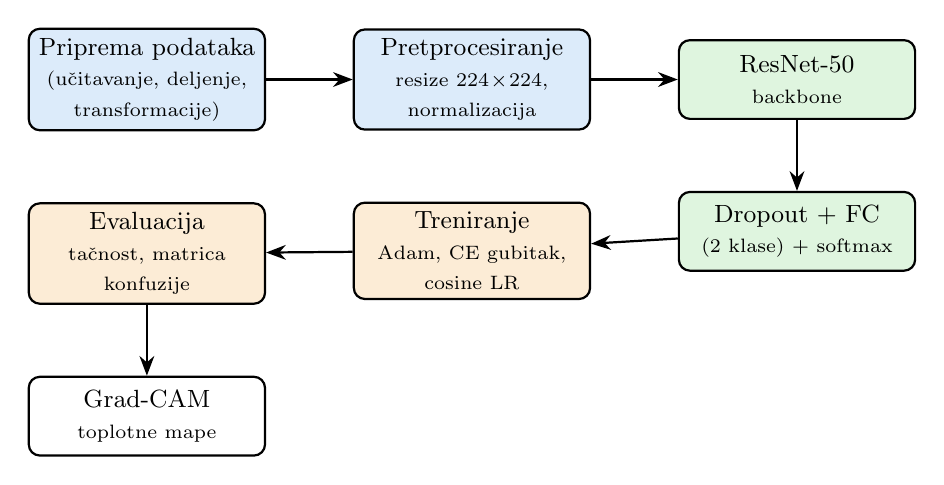
\begin{tikzpicture}[
    node distance=0.9cm and 1.1cm,
    blok/.style={rectangle,rounded corners,draw,thick,minimum width=3.0cm,
                 minimum height=1.0cm,align=center,fill=blokplava,font=\small},
    blokz/.style={blok,fill=blokzelena},
    blokn/.style={blok,fill=bloknarandzasta},
    strelica/.style={-{Stealth[length=2.5mm]},thick}
]
\node[blok] (data) {Priprema podataka\\\scriptsize (učitavanje, deljenje,\\\scriptsize transformacije)};
\node[blok,right=of data] (pre) {Pretprocesiranje\\\scriptsize resize $224\!\times\!224$,\\\scriptsize normalizacija};
\node[blokz,right=of pre] (cnn) {ResNet-50\\\scriptsize backbone};
\node[blokz,below=of cnn] (head) {Dropout + FC\\\scriptsize (2 klase) + softmax};
\node[blokn,below=of pre] (train) {Treniranje\\\scriptsize Adam, CE gubitak,\\\scriptsize cosine LR};
\node[blokn,below=of data] (eval) {Evaluacija\\\scriptsize tačnost, matrica\\\scriptsize konfuzije};
\node[blok,below=of eval,fill=white] (cam) {Grad-CAM\\\scriptsize toplotne mape};

\draw[strelica] (data) -- (pre);
\draw[strelica] (pre) -- (cnn);
\draw[strelica] (cnn) -- (head);
\draw[strelica] (head) -- (train);
\draw[strelica] (train) -- (eval);
\draw[strelica] (eval) -- (cam);
\end{tikzpicture}
\caption{Blok-dijagram celokupnog sistema za klasifikaciju MRI preseka lumbalne kičme.}
\label{fig:blokdijagram}
\end{figure}

\subsection{Baza podataka}
\label{sec:baza}

Korišćen je javno dostupan skup podataka \textit{Lumbar Spinal MRI
Dataset}~\cite{khan2023dataset}, dostupan na platformi Kaggle na adresi:\\
\url{https://www.kaggle.com/datasets/abdullahkhan70/lumbar-spinal-mri-dataset}.

Skup sadrži aksijalne MRI preseke lumbalne kičme organizovane u tri originalne
kategorije: \textit{Herniated Disc} (hernija diska), \textit{No Stenosis} (uredan nalaz,
bez stenoze) i \textit{Thecal Sac}. U ovom radu klasa \textit{Thecal Sac} je izostavljena
jer ne predstavlja dijagnostičku kategoriju uporedivu sa preostale dve, te je problem
sveden na \textbf{binarnu klasifikaciju} (hernija diska naspram urednog nalaza). Podaci
su unapred podeljeni u \texttt{train} i \texttt{test} foldere; raspodela broja snimaka po
klasama data je u tabeli~\ref{tab:baza}.

\begin{table}[H]
\centering
\caption{Broj snimaka po klasama u korišćenom skupu podataka (nakon izostavljanja klase
\textit{Thecal Sac}).}
\label{tab:baza}
\begin{tabular}{lccc}
\toprule
\textbf{Klasa} & \textbf{train folder} & \textbf{test folder} & \textbf{Ukupno} \\
\midrule
Hernija diska (Herniated Disc) & 3063 & 1218 & 4281 \\
Uredan nalaz (No Stenosis)     & 3152 & 1507 & 4659 \\
\midrule
\textbf{Ukupno}                & 6215 & 2725 & 8940 \\
\bottomrule
\end{tabular}
\end{table}

Validacioni skup formiran je objedinjavanjem $15\%$ stratifikovano izdvojenih snimaka iz
\texttt{train} foldera i snimaka iz \texttt{test} foldera, dok je preostalih $85\%$
\texttt{train} foldera korišćeno za treniranje. Primeri snimaka iz obe klase prikazani su
na slici~\ref{fig:primeri}.

\begin{figure}[H]
\centering
\placeholderbox{5cm}{Reprezentativni aksijalni MRI preseci: levo --- hernija diska,
desno --- uredan nalaz. (Slika se generiše skriptom opisanom u prilogu; videti
uputstvo za reprodukciju.)}
\caption{Reprezentativni primeri ulaznih snimaka iz dve klase.}
\label{fig:primeri}
\end{figure}

\subsection{Pretprocesiranje}
\label{sec:preproc}

Svaki snimak se skalira na rezoluciju $224\times224$ piksela i konvertuje u tenzor, nakon
čega se normalizuje po kanalima korišćenjem standardnih ImageNet~\cite{deng2009imagenet}
statistika (srednje vrednosti $[0{,}485;\,0{,}456;\,0{,}406]$ i standardne devijacije
$[0{,}229;\,0{,}224;\,0{,}225]$). Ista transformacija primenjuje se na trening,
validacioni i test skup. Zbog blage neuravnoteženosti klasa, u funkciji gubitka koriste
se težine klasa (videti jednačinu~\ref{eq:ce}).

\subsection{Arhitektura klasifikatora}
\label{sec:arh}

Kao osnova (\textit{backbone}) koristi se ResNet-50~\cite{he2016deep}. Originalni
klasifikacioni sloj zamenjen je sekvencom koja se sastoji od \textit{dropout} sloja
(verovatnoća $0{,}3$) i potpuno povezanog (\textit{fully-connected}) sloja sa dva izlaza,
po jedan za svaku klasu. Mreža se trenira \textit{od nule} (bez ImageNet predtreniranih
težina), čime se ispituje sposobnost arhitekture da nauči obeležja specifična za MRI
domen direktno iz dostupnih podataka.

\subsection{Treniranje}
\label{sec:trening}

Treniranje je izvedeno na iznajmljenom grafičkom procesoru \textbf{NVIDIA RTX 4090
(24\,GB)} preko platforme \textit{vast.ai}. Korišćeni hiperparametri sumirani su u
tabeli~\ref{tab:hiperparametri}. Optimizacija se vrši algoritmom Adam~\cite{kingma2015adam}
uz kosinusno opadanje stope učenja~\cite{loshchilov2017sgdr} tokom svih epoha. Radi
stabilnosti treniranja primenjeno je odsecanje norme gradijenta (engl.\ \textit{gradient
clipping}) na vrednost $1{,}0$, a tokom treniranja praćena je i prosečna norma gradijenta
po epohi. Model sa najboljom tačnošću na validacionom skupu čuva se kao finalni model.

\begin{table}[H]
\centering
\caption{Hiperparametri treniranja.}
\label{tab:hiperparametri}
\begin{tabular}{ll}
\toprule
\textbf{Hiperparametar} & \textbf{Vrednost} \\
\midrule
Arhitektura            & ResNet-50 (od nule) \\
Ulazna rezolucija      & $224\times224$ \\
Broj epoha             & 200 \\
Veličina batch-a       & 128 \\
Optimizator            & Adam \\
Početna stopa učenja   & $5\times10^{-4}$ \\
Raspored stope učenja  & Cosine annealing \\
Weight decay ($L_2$)   & $5\times10^{-4}$ \\
Dropout                & $0{,}3$ \\
Funkcija gubitka       & Težinska unakrsna entropija \\
Gradient clipping      & $1{,}0$ \\
Seed                   & 42 \\
\bottomrule
\end{tabular}
\end{table}

\subsection{Evaluacija i metrike}
\label{sec:metrike}

Kvalitet modela meri se na test skupu pomoću tačnosti (engl.\ \textit{accuracy}),
senzitivnosti (engl.\ \textit{sensitivity}/\textit{recall}), specifičnosti (engl.\
\textit{specificity}) i površine ispod ROC krive (AUC), uz prikaz matrice konfuzije. Za
pozitivnu klasu uzima se \textit{hernija diska}. Metrike se računaju na sledeći način:
\begin{equation}
\text{Acc}=\frac{TP+TN}{TP+TN+FP+FN},\quad
\text{Sens}=\frac{TP}{TP+FN},\quad
\text{Spec}=\frac{TN}{TN+FP}.
\label{eq:metrike}
\end{equation}
Nakon evaluacije, na odabranim primerima primenjuje se Grad-CAM
(odeljak~\ref{sec:teorija}) radi vizuelne provere da li se model fokusira na anatomski
relevantne regione.

% ===========================================================================
% 3. REZULTATI SA DISKUSIJOM
% ===========================================================================
\section{Rezultati sa diskusijom}
\label{sec:rezultati}

\subsection{Tok treniranja}
\label{sec:krive}

Na slici~\ref{fig:krive} prikazane su krive treniranja: gubitak (levo) i tačnost
(sredina) za trening i validacioni skup, kao i prosečna norma gradijenta po epohi
(desno). Krive pokazuju očekivano opadanje gubitka i porast tačnosti tokom treniranja,
dok norma gradijenta ostaje stabilna zahvaljujući odsecanju gradijenta.

\begin{figure}[H]
\centering
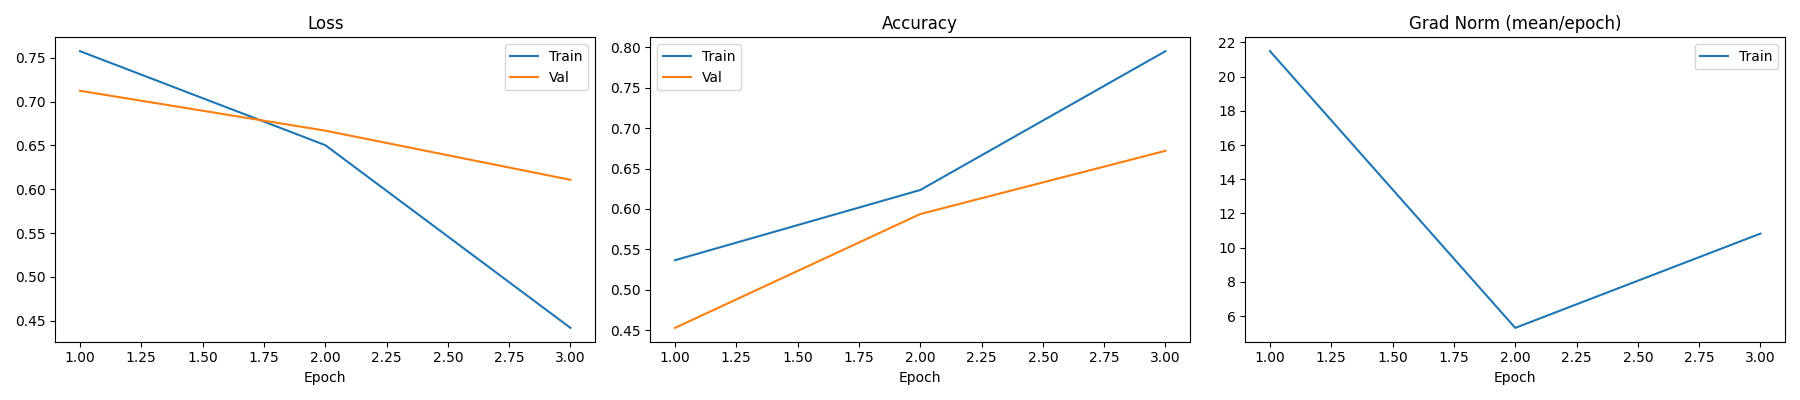
\includegraphics[width=\linewidth]{figures/learning_curves.png}
\caption{Krive treniranja: gubitak, tačnost i prosečna norma gradijenta po epohi za
trening i validacioni skup.}
\label{fig:krive}
\end{figure}

\subsection{Konačni rezultati}
\label{sec:finalni}

Sumarni rezultati na test skupu prikazani su u tabeli~\ref{tab:rezultati}, a matrica
konfuzije na slici~\ref{fig:konfuzija}. \textit{(Numeričke vrednosti su ostavljene kao
rezervisana mesta i popunjavaju se nakon evaluacije istreniranog modela.)}

\begin{table}[H]
\centering
\caption{Rezultati klasifikacije na test skupu. Pozitivna klasa: hernija diska.}
\label{tab:rezultati}
\begin{tabular}{lc}
\toprule
\textbf{Metrika} & \textbf{Vrednost} \\
\midrule
Tačnost (Accuracy)        & [XX{,}X\%] \\
Senzitivnost (Sensitivity)& [XX{,}X\%] \\
Specifičnost (Specificity)& [XX{,}X\%] \\
Preciznost (Precision)    & [XX{,}X\%] \\
F1 mera                   & [0{,}XX] \\
AUC                       & [0{,}XX] \\
\bottomrule
\end{tabular}
\end{table}

\begin{figure}[H]
\centering
\placeholderbox{6cm}{Matrica konfuzije (2$\times$2) na test skupu, sa apsolutnim brojem i
procentom za svako polje. (Generiše se skriptom za evaluaciju; videti uputstvo za
reprodukciju.)}
\caption{Matrica konfuzije na test skupu.}
\label{fig:konfuzija}
\end{figure}

\subsection{Vizuelizacija pomoću Grad-CAM metode}
\label{sec:gradcam-rez}

Na slici~\ref{fig:gradcam} prikazane su Grad-CAM toplotne mape za reprezentativne uzorke
iz trening i test skupa. Za svaki uzorak prikazani su ulazni snimak (levo), toplotna mapa
značajnosti (sredina) i njihova superpozicija (desno), zajedno sa tačnom i predviđenom
klasom. Uočava se da se kod ispravno klasifikovanih primera aktivacije pretežno
koncentrišu u regionu intervertebralnog diska i duralne vreće, što je u skladu sa
anatomskim kriterijumima dijagnostike i sa zapažanjima iz literature~\cite{hou2023mri}.

\begin{figure}[H]
\centering
\includegraphics[width=0.85\linewidth]{figures/gradcam_summary.png}
\caption{Grad-CAM vizuelizacije za reprezentativne uzorke (kolone: ulaz, toplotna mapa,
superpozicija). Iznad svakog reda navedeni su tačna i predviđena klasa.}
\label{fig:gradcam}
\end{figure}

\subsection{Analiza promašaja}
\label{sec:promasaji}

Na slici~\ref{fig:promasaj} prikazani su tipični primeri pogrešno klasifikovanih snimaka.
Greške se najčešće javljaju kod graničnih slučajeva blage protruzije diska, kao i kod
snimaka sa izraženim artefaktima ili netipičnom orijentacijom. Grad-CAM mape kod
promašaja često pokazuju rasute ili pomerene aktivacije van regiona diska, što ukazuje na
to da model u tim slučajevima nije izdvojio dijagnostički relevantno obeležje.

\begin{figure}[H]
\centering
\placeholderbox{5cm}{Primeri pogrešno klasifikovanih snimaka sa pripadajućim Grad-CAM
mapama i obrazloženjem (granični slučajevi, artefakti). Bira se iz izlaza skripte za
Grad-CAM gde je \texttt{pred} $\neq$ \texttt{true}.}
\caption{Primeri promašaja modela uz Grad-CAM objašnjenje.}
\label{fig:promasaj}
\end{figure}

\subsection{Poređenje sa literaturom}
\label{sec:poredjenje}

U tabeli~\ref{tab:poredjenje} naši rezultati upoređeni su sa rezultatima Hou i
saradnika~\cite{hou2023mri}. Treba imati u vidu da poređenje nije potpuno direktno: oni
koriste polu-nadgledano kontrastivno predtreniranje i višeslojni ulaz (tri susedna
aksijalna preseka), dok mi koristimo jednostavniji, potpuno nadgledani pristup sa jednim
presekom i mrežom treniranom od nule. Uprkos tome, dobijene vrednosti su uporedive, što
sugeriše da i direktan CNN klasifikator može da postigne kliničkog interesantne rezultate
na ovom zadatku.

\begin{table}[H]
\centering
\caption{Poređenje sa rezultatima iz literature.}
\label{tab:poredjenje}
\begin{tabular}{lcccc}
\toprule
\textbf{Metod} & \textbf{Tačnost} & \textbf{Senzitivnost} & \textbf{Specifičnost} & \textbf{AUC} \\
\midrule
Hou i sar.~\cite{hou2023mri} (polu-nadgledano) & $87{,}11\%$ & $87{,}50\%$ & $86{,}72\%$ & $0{,}9487$ \\
Naš model (ResNet-50, nadgledano)              & [XX{,}X\%]  & [XX{,}X\%]  & [XX{,}X\%]  & [0{,}XX] \\
\bottomrule
\end{tabular}
\end{table}

\paragraph{Diskusija.}
Glavne sličnosti sa literaturom su izbor aksijalnih preseka kao ulaza i upotreba
toplotnih mapa za interpretaciju. Glavne razlike su u složenosti metode: naš pristup je
jednostavniji za implementaciju i ne zahteva fazu samonadgledanog predtreniranja, ali je
zato osetljiviji na količinu i kvalitet označenih podataka. Korišćenje samo jednog
preseka umesto tri susedna potencijalno gubi deo informacije u vertikalnom pravcu, što
može objasniti eventualne razlike u performansama na graničnim slučajevima.

% ===========================================================================
% 4. ZAKLJUČAK
% ===========================================================================
\section{Zaključak}
\label{sec:zakljucak}

U ovom radu predstavljen je sistem za binarnu klasifikaciju aksijalnih MRI preseka
lumbalne kičme u kategorije hernija diska i uredan nalaz, zasnovan na konvolucionoj
neuronskoj mreži ResNet-50. Pokazano je da relativno jednostavan, potpuno nadgledani
pristup postiže rezultate uporedive sa složenijom polu-nadgledanom metodom iz
literature~\cite{hou2023mri}. Primenom Grad-CAM metode potvrđeno je da se model pretežno
fokusira na anatomski relevantne regione, čime se povećava poverenje u njegove odluke i
omogućava lakše otkrivanje uzroka grešaka.

\paragraph{Smernice za budući rad.}
Kao pravci daljeg istraživanja izdvajaju se: (i) korišćenje predtreniranih težina
(transfer učenje) i augmentacije podataka radi poboljšanja generalizacije; (ii) prelazak
sa jednog na više susednih aksijalnih preseka, po uzoru na~\cite{hou2023mri}, radi
uključivanja vertikalne informacije; (iii) proširenje na više klasa (npr.\ stepenovanje
težine stenoze) i (iv) kvantitativna evaluacija kvaliteta Grad-CAM mapa u saradnji sa
radiologom.

% ===========================================================================
% LITERATURA
% ===========================================================================
\newpage
\bibliographystyle{ieeetr}
\bibliography{references}

\end{document}
